% Copyright 2013 Nicolai Hähnle <nhaehnle@gmail.com>
%
% This work is licensed under the Creative Commons Attribution-ShareAlike 3.0
% Unported License, see http://creativecommons.org/licenses/by-sa/3.0/
% 
% Among other things, this means that yes, you may take e.g. illustrations from
% the book and use them in your own work. However, (a) you must give proper
% attribution by naming me as its original author and (b) you must make your
% derivative work available under the same or similar license terms.
%
% See the Creative Commons website for the exact licensing terms.

\chapter{Reduced bases, the LLL algorithm, and approximating shortest vectors}
\label{chapter:basis-reduction-LLL}

In this chapter, we will see the lattice basis reduction algorithm due to
Lenstra, Lenstra, and Lovász~\cite{MR682664}, which we will use to approximate the shortest
vector problem.

Imagine being given a lattice basis $B \in \Q^{d \times d}$.\footnote{We
restrict our attention to rational numbers because it is unclear how to deal with arbitrary real numbers
on a computer. With some care, many but not all statements can be extended to theoretical models of computation
that allow computation with real numbers, but we will not address those questions here.}
The simplest and stupidest thing you could possibly do to approximate a shortest vector in $\Lambda(B)$
is to just return the shortest vector of this basis.
If the basis vectors are orthogonal, you will even find a shortest lattice vector
in this way.
This should be clear intuitively:
\begin{center}
  \begin{tikzpicture}
    \fill (0,0) circle (2pt) node[below left] {$0$};
    \draw[thick,->] (0,0) -- (4,0) node[below] {$b_2$};
    \draw[thick,->] (0,0) -- (0,2) node[left] {$b_1$};
  \end{tikzpicture}
\end{center}
Let us solidify our intuition formally.
For every lattice vector $x \in \Lambda(B)$,
we have
\[
  \|x\|_2^2 = \|a_1b_1 + \dots + a_db_d\|_2^2 = a_1^2 \|b_1\|_2^2 + \dots + a_d^2 \|b_d\|_2^2 \geq \|b_k\|_2^2,
\]
where $a_j \in \Z$ for all $j$,
and the last inequality holds for any $k$ with $a_k \neq 0$.
This gives us a lower bound on the length of any non-zero lattice vector,
and it just so happens that this lower bound coincides with the length of a shortest vector in the given basis.

We can extend at least part of this argument to non-orthogonal bases.
Consider the following situation:
\begin{center}
  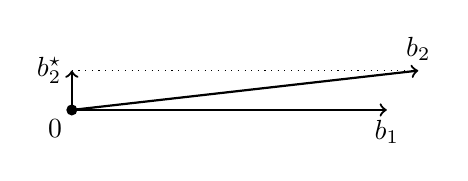
\begin{tikzpicture}
    \fill (0,0) circle (2pt) node[below left] {$0$};
    \draw[thick,->] (0,0) -- (4,0) node[below] {$b_1$};
    \draw[thick,->] (0,0) -- (4.4,0.5) node[above] {$b_2$};
    \draw[thick,->] (0,0) -- (0.0,0.5) node[left] {$b_2^\star$};
    \draw[dotted] (0,0.5) -- (4.4,0.5);
  \end{tikzpicture}
\end{center}
Every non-zero lattice vector $x$ lies either on the line $\langle b_1 \rangle$ through $b_1$,
in which case its length is at least $\|b_1\|_2$;
or it lies on a line parallel to $\langle b_1 \rangle$.
However, every such line that contains a lattice point has distance at least $\|b_2^\star\|_2$
from the origin, where $b_2^\star = \pi_1(b_2)$ is the orthogonal projection of $b_2$
onto the orthogonal complement of $\langle b_1 \rangle$.

So $\ell := \min\{\|b_1\|_2, \|b_2^\star\|_2\}$ is a lower bound on the length $\lambda_1$
of a non-zero lattice vector.
This means that we can prove an approximation ratio of $\frac{\|b_1\|_2}{\ell}$
for the simple algorithm that just returns the first lattice basis vector.
Unfortunately, this ratio can be arbitrarily large depending on the given basis.

We will first formalize the preceding ideas using the Gram-Schmidt orthogonalization of a basis,
and will then discuss ways of finding a ``good'' basis in the sense that the resulting approximation ratio
is bounded. As the picture suggests, ``good'' in this context entails ``close to orthogonal''.



\section{Gram-Schmidt orthogonalization}

\begin{definition}
  Let $B = (b_1, \ldots, b_r) \in \R^{d \times r}$ be a lattice basis.
  Its \emph{Gram-Schmidt orthogonalization} $B^\star = (b_1^\star, \ldots, b_r^\star) \in \R^{d \times r}$
  is defined via
  \[
    b_k^\star := \pi_{k-1}(b_k)
      = b_k - \sum_{j=1}^{k-1} \underbrace{\frac{{b_k}^T b_j^\star}{{b_j^\star}^T b_j^\star}}_{=: \mu_{jk}} b_j^\star
  \]
  Recall that $\pi_{k-1} : \R^d \to \langle b_1, \ldots, b_{k-1} \rangle$ is the orthogonal projection
  onto the orthogonal complement of the space spanned by $b_1, \ldots, b_{k-1}$.
\end{definition}
\begin{lemma}
  $B^\star$ is orthogonal, that is, ${b_j^\star}^T b_k^\star = 0$ for all $j \neq k$.
\end{lemma}
\begin{proof}
  Given $j < k$, we simply compute, using the definition of $b_k^\star$:
  \begin{align*}
    {b_j^\star}^T b_k^\star
      &= {b_j^\star}^T b_k - \sum_{i=1}^{k-1} \mu_{ik} \underbrace{{b_j^\star}^T b_i^\star}_{= 0 \text{ for } j \neq i} \\
      &= {b_j^\star}^T b_k - \mu_{jk} {b_j^\star}^T b_j^\star \\
      &= {b_j^\star}^T b_k - \frac{b_k^T b_j^\star}{{b_j^\star}^T b_j^\star} {b_j^\star}^T b_j^\star = 0
  \end{align*}
  To make the second step work, we proceed by induction first over $k$ and then over $j < k$.
\end{proof}

We will often use the definition in its rearranged form:
\[
  b_k = b_k^\star + \sum_{j < k} \mu_{jk} b_j^\star
\]
We often use this set of equations for $k = 1\dots r$ in matrix form:
\[
  B = B^\star M, \text{ where } M = \begin{pmatrix}
                                      1 & \mu_{12} & \dots  & \mu_{1r} \\
                                      0 &    1     &        & \\
                                      \vdots &     & \ddots & \vdots \\
                                      0 &          &        &   1
                                    \end{pmatrix}
\]
Let us formalize the discussion at the beginning of this chapter.
\begin{lemma}
  \label{lemma:svp-lower-bound-gso}
  For all $x \in \Lambda(B) \setminus \{0\}$ we have $\|x\|_2 \geq \min_j \|b_j^\star\|_2$.
\end{lemma}
\begin{proof}
  By definition, we can write $x = a_1 b_1 + \dots + a_r b_r$,
  where $a_j \in \Z$ and there is at least one $a_j \neq 0$.
  In fact, we can write
  \[
    x = a_1 b_1 + \dots + a_k b_k
  \]
  where $k$ is the \emph{last} index with $a_k \neq 0$.
  Now, we compute a change of basis to $B^\star$:
  \begin{align*}
    x &= (a_1 + \mu_{12} a_2 + \dots + \mu_{1k} a_k) b_1^\star \\
      &+ (a_2 + \mu_{23} a_3 + \dots + \mu_{2k} a_k) b_2^\star \\
      &+ \dots \\
      &+ (a_{k-1} + \mu_{k-1,k} a_k) b_{k-1}^\star \\
      &+ a_k b_k^\star
  \end{align*}
  Using Pythagoras' theorem, it follows that
  \begin{align*}
    \|x\|_2 &\geq |a_k| \|b_k^\star\|_2 \geq \|b_k^\star\|_2 \geq \min_j \|b_j^\star\|_2 \qedhere
  \end{align*}
\end{proof}



\section{Reduced bases}

Recall the example basis from the beginning of the chapter,
and recall the observations from the proof of Lemma~\ref{lemma:every-lattice-has-basis}
about lattice points in a certain ``corridor'' around the orthogonal complement of $b_1$.
This immediately suggests that we can get a ``better'', more orthogonal basis
by replacing $b_2$ by $b_2 - b_1$ without changing the lattice:
\begin{center}
  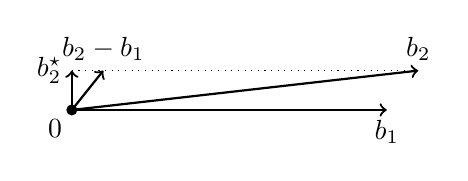
\begin{tikzpicture}
    \fill (0,0) circle (2pt) node[below left] {$0$};
    \draw[thick,->] (0,0) -- (4,0) node[below] {$b_1$};
    \draw[thick,->] (0,0) -- (4.4,0.5) node[above] {$b_2$};
    \draw[thick,->] (0,0) -- (0.4,0.5) node[above] {$b_2 - b_1$};
    \draw[thick,->] (0,0) -- (0.0,0.5) node[left] {$b_2^\star$};
    \draw[dotted] (0,0.5) -- (4.4,0.5);
  \end{tikzpicture}
\end{center}
Visual inspection tells us that $b_2 - b_1$ is a shortest vector.
However, we can get an even more orthogonal basis:
note that this new vector is shorter than $\|b_1\|$,
and if we exchange the two basis vector, the new orthogonalization suggests another ``size reduction'' step:
\begin{center}
  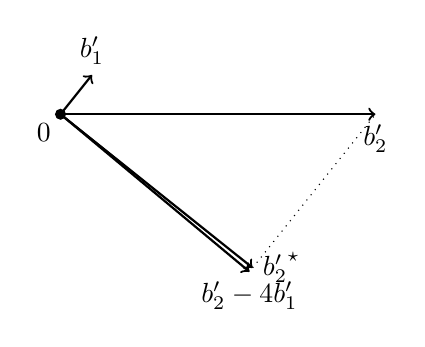
\begin{tikzpicture}
    \fill (0,0) circle (2pt) node[below left] {$0$};
    \draw[thick,->] (0,0) -- (4,0) node[below] {$b_2'$};
    \draw[thick,->] (0,0) -- (0.4,0.5) node[above] {$b_1'$};
    \draw[thick,->] (0,0) -- (2.44,-1.95) node[right] {${b_2'}^\star$};
    \draw[dotted] (2.44,-1.95) -- (4,0);
    \draw[thick,->] (0,0) -- (2.4,-2) node[below] {$b_2' - 4b_1'$};
  \end{tikzpicture}
\end{center}
Surprise: the lattice has an almost exactly orthogonal basis!

The two types of operations we have performed to get to a better basis
suggest a definition of a ``good'' basis as one where these operations can no longer be performed:
\begin{definition}[$d=2$]
  \label{def:reduced-basis-2dim}
  A basis $B \in \R^{d\times 2}$ of a two-dimensional lattice is \emph{reduced} if
  \begin{enumerate}
    \item $|\mu_{12}| \leq 1/2$ (so called \emph{size-reducedness}) and
    \item $\|b_1\|_2 \leq \|b_2\|_2$.
  \end{enumerate}
\end{definition}
Let us contemplate what a reduced basis buys us.
\begin{center}
  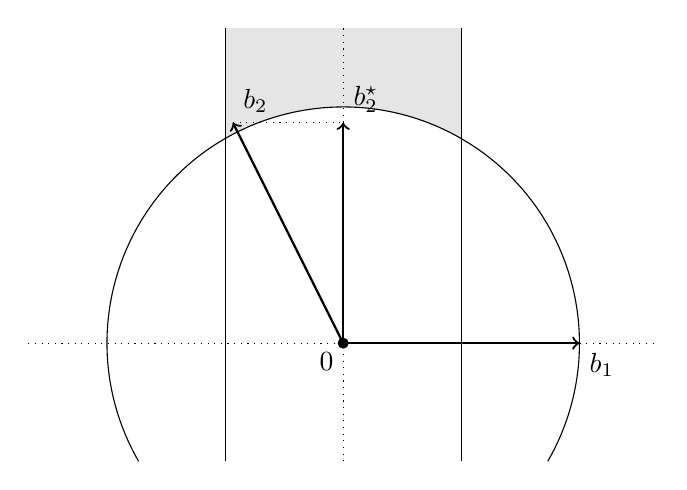
\begin{tikzpicture}
    \fill[black!10] (-1.5,4) -- (120:3cm) arc[start angle=120, end angle=60, radius=3cm] -- (1.5,4);
    \draw[dotted] (-4,0) -- (4,0);
    \draw[dotted] (0,-1.5) -- (0,4);
    \fill (0,0) circle (2pt) node[below left] {$0$};
    \draw[thick,->] (0,0) -- (3,0) node[below right] {$b_1$};
    \draw (-30:3cm) arc[start angle=-30,end angle=210,radius=3cm];
    \draw (1.5,-1.5) -- (1.5,4);
    \draw (-1.5,-1.5) -- (-1.5,4);

    \draw[dotted] (-1.4,2.8) -- (0,2.8);
    \draw[thick,->] (0,0) -- (-1.4,2.8) node[above right] {$b_2$};
    \draw[thick,->] (0,0) -- (0,2.8) node[above right] {$b_2^\star$};
  \end{tikzpicture}
\end{center}
The definition of reduced basis implies that $b_2$ must lie in the shaded region
(or its mirror image that points down).
With this picture in mind, it is not difficult to show that $b_1$ is a shortest lattice vector.

For our purposes and with Lemma~\ref{lemma:svp-lower-bound-gso} in mind,
it is interesting to see that $b_2^\star$ can be shorter than $b_1$, but not by much:
\begin{fact}
  \label{fact:reduced-basis-2dim-size-bound}
  In a reduced basis, $\|b_2^\star\|_2 \geq \sqrt{3/4} \|b_1\|_2$.
\end{fact}
\begin{proof}
  Writing $b_2 = b_2^\star + \mu_{12} b_1^\star$, taking squares,
  and remembering that $b_1 = b_1^\star$,
  the second condition of Definition~\ref{def:reduced-basis-2dim} becomes
  \[
    \|b_1^\star\|_2^2 \leq \|b_2^\star + \mu_{12} b_1^\star\|_2^2 = \|b_2^\star\|_2^2 + \mu_{12}^2 \|b_1^\star\|_2^2
  \]
  Rearranging, we get
  \[
    \|b_2^\star\|_2^2 \geq (1 - \mu_{12}^2) \|b_1^\star\|_2^2 \geq \frac{3}{4} \|b_1^\star\|_2^2,
  \]
  where the second inequality follows from the first condition of Definition~\ref{def:reduced-basis-2dim}.
  Now we simply take square roots again to obtain the result.
\end{proof}
The proof of this fact suggests the following non-trivial generalization of
Definition~\ref{def:reduced-basis-2dim} to arbitrary dimension:
\begin{definition}
  A lattice basis is \emph{reduced} if
  \begin{enumerate}
    \item $|\mu_{ij}| \leq 1/2$ for all $i < j$ and
    \item $\|b_j^\star\|_2^2 \leq \|b_{j+1}^\star + \mu_{j,j+1} b_j^\star\|_2^2$ for all $j$ within range.
  \end{enumerate}
\end{definition}

\begin{remark}
  The definitions of reduced bases coincide for $d = 2$.
  Furthermore, the definition can be understood as saying that every ``block''
  of adjacent basis vectors is reduced in the sense that the vectors
  $\pi_{j-1}(b_j), \pi_{j-1}(b_{j+1})$ form a reduced basis of a certain $2$-dimensional lattice.
  This perspective leads to a generalized notion of
  basis reduction that has been studied by Schnorr~\cite{MR918090}.
\end{remark}

\begin{lemma}
  \label{lemma:size-bounds-reduced-basis}
  In a reduced basis $B$ of a lattice of dimension $r$, one has:
  \begin{enumerate}
    \item $\|b_{j+1}^\star\|_2 \geq \sqrt{3/4} \|b_j^\star\|_2$,
    \item $\|b_j^\star\|_2 \geq (3/4)^{(j-1)/2} \|b_1\|_2$, and
    \item $b_1$ is a $(4/3)^{(r-1)/2}$-approximation to a shortest non-zero vector of $\Lambda(B)$.
  \end{enumerate}
\end{lemma}
\begin{proof}
  The first statement is analogous to the proof of Fact~\ref{fact:reduced-basis-2dim-size-bound},
  and the second statement follows from the first by induction on $j$.

  The last statement combines the second statement with Lemma~\ref{lemma:svp-lower-bound-gso}:
  Let $x \in \Lambda(B) \setminus \{ 0 \}$.
  We can compute
  \[
    \|x\|_2 \geq \min_j \|b_j^\star\|_2 \geq \min_j (3/4)^{(j-1)/2} \|b_1\|_2 = (3/4)^{(r-1)/2} \|b_1\|_2.
  \]
  Rearranging, we get that
  \[
    \|b_1\|_2 \leq (4/3)^{(r-1)/2} \|x\|_2
  \]
  for all $x \in \Lambda(B) \setminus \{ 0 \}$.
  In particular, the inequality holds when $x$ is a shortest non-zero vector of $\Lambda(B)$,
  which is exactly the definition of an approximation.
\end{proof}

In the next sections, we will address the question
whether reduced bases always exist and whether we can compute them efficiently.



\section{The determinant of general lattices}
\label{sec:determinant-general-lattices}

Previously, we defined the determinant of a full-dimensional lattice $\Lambda$
as $\det \Lambda = |\det B|$ for some basis $B$ of $\Lambda$,
and we saw that $\det \Lambda = \vol \cP_B$.
We would like a definition of the determinant of a general lattice that coincides
with the definition we already have.
The definitions should coincide not only in the sense that they are equal for full-dimensional lattices,
but also in the sense that we get the same answer for $\Lambda \subset \R^d$
and for $\tau(\Lambda) \subset \R^r$ where $r = \dim\Lambda$ and $\tau$ is an orthogonal transformation
(that is, a transformation that preserves scalar products).

\begin{lemma}
  \label{lemma:determinant-b-star-full-dim}
  Let $B \in \R^{d \times d}$ be a basis of a full-dimensional lattice $\Lambda$.
  Then $\det \Lambda = \prod_{j=1}^d \|b_j^\star\|_2$.
\end{lemma}
\begin{proof}
  Geometrically, this is true because Gram-Schmidt orthogonalization transforms
  the fundamental parallelepiped $\cP_B$ into an \emph{orthogonal} parallelepiped $\cP_{B^\star}$
  with side lengths $\|b_j^\star\|_2$
  by a sequence of shearing operations that leave the volume unchanged.

  More formally, we can write $B = B^\star M$, where $M$ is upper triangular with $1$s on the diagonal.
  Hence $\det B = \det B^\star$. We compute
  \[
    (\det B^\star)^2 = \det {B^\star}^T B^\star = \det \begin{pmatrix}
        \|b_1^\star\|_2^2 &        & 0 \\
                          & \ddots &   \\
        0                 &        & \|b_d^\star\|_2^2
      \end{pmatrix} = \prod_j \|b_j^\star\|_2^2
  \]
  and the claim follows.
\end{proof}

\begin{definition}
  Let $\Lambda \subset \R^d$ be a lattice of dimension $r$.
  Its \emph{determinant} is given by $\det\Lambda := \sqrt{\det(B^TB)}$
  where $B \in \R^{d \times r}$ is a basis of $\Lambda$.
\end{definition}

To see that this definition is well-defined, let $B' \in \R^{d \times r}$ be another basis of $\Lambda$.
By the discussion around Lemma~\ref{lemma:basis-exchange-is-unimodular},
there is a unimodular matrix $U \in \Z^{r \times r}$ such that $B = B'U$.
We can compute
\[
  \det(B^T B) = \det(\underbrace{U^T}_{r \times r} \underbrace{{B'}^T B'}_{r \times r} \underbrace{U}_{r \times r})
    = \underbrace{\det(U)^2}_{=1} \det({B'}^T B') = \det({B'}^T B')
\]
That is, the definition of determinant does not depend on the choice of basis.

\begin{lemma}
  \label{lemma:determinant-b-star}
  Let $B \in \R^{d \times r}$ be a basis of the lattice $\Lambda$.
  Then $\det \Lambda = \prod_{j=1}^r \|b_j^\star\|_2$.
\end{lemma}
\begin{proof}
  The proof is analogous to the proof of Lemma~\ref{lemma:determinant-b-star-full-dim}.
\end{proof}

The norms $\|b_j^\star\|_2$ are invariant under orthogonal transformations,
and so this Lemma is one way to confirm that our original goal has been reached:
the new definition of the determinant of a lattice $\Lambda \subseteq \R^d$ of dimension $r$
is equal to the determinant that we obtain according to the original definition
after embedding $\Lambda$ into $\R^r$ by an orthogonal transformation.




\section{Existence of reduced bases}

Let us consider the following stylized algorithm for basis reduction:
\begin{codebox}
  \Procname{$\proc{Reduce}(B \in \Z^{d \times d})$}
  \li Perform size reduction: ensure $|\mu_{ij}| \leq 1/2$ for all $i < j$ without changing $\Lambda(B)$
  \li \If $\exists j: \|b_j^\star\|_2^2 > \|b_{j+1}^\star + \mu_{j,j+1} b_j^\star\|_2^2$
  \li \Then Swap $b_j \leftrightarrow b_{j+1}$
  \li       \Goto 1.
      \End
  \li \Return $B$
\end{codebox}
It is clear by construction that \emph{if} \proc{Reduce} terminates,
it has computed a reduced basis.
To show \emph{that} \proc{Reduce} terminates,
we analyze the potential function
\begin{align*}
  \Phi(B) &:= \prod_{j=1}^d \prod_{i=1}^j \|b_i^\star\|_2^2 \\
          &= \prod_{j=1}^d (\det \Lambda_j)^2,
\end{align*}
where $\Lambda_j := \Lambda(b_1,\ldots,b_j)$.
\begin{lemma}
  $\Phi(B) \in \N_{\geq 1}$.
\end{lemma}
\begin{proof}
  By definition, $(\det\Lambda_j)^2 = \det(B_j^T B_j)$,
  where $B_j \in \Z^{d \times j}$ contains the first $j$ columns of $B$.
  So $(\det\Lambda_j)^2$ is a positive integer, and the same holds for the product $\Phi(B)$.
\end{proof}

We leave a precise analysis of the size reduction step as an exercise.
For now, it suffices to know that size reduction performs a sequence
of elementary basis transformations of the form: replace $b_j$ by $b_j + \alpha b_i$,
where $i < j$ and $\alpha \in \Z$.\footnote{$\alpha$ is chosen so that $|\mu_{ij}| \leq 1/2$ after the transformation.}
Such transformations do not change the $\Lambda_j$ for any $j$, and therefore:

\begin{lemma}
  $\Phi(B)$ is not changed by size reduction.
\end{lemma}

\begin{lemma}
  \label{lemma:reduce-phi-decreases}
  $\Phi(B)$ strictly decreases every time line~3 of \proc{Reduce} executes.
\end{lemma}
\begin{proof}
  Let us denote by $B$ and $B'$ the lattice bases before and after the swap of $b_j$ and $b_{j+1}$,
  respectively.
  First, note that $\Lambda_i = \Lambda_i'$ for all $i \neq j$, so that
  \[
    \frac{\Phi(B')}{\Phi(B)} = \frac{(\det\Lambda_j')^2}{(\det\Lambda_j)^2}
      = \frac{\prod_{i=1}^j \|{b_i'}^\star\|_2^2}{\prod_{i=1}^j \|{b_i}^\star\|_2^2}
      = \frac{\|{b_j'}^\star\|_2^2}{\|{b_j}^\star\|_2^2}
  \]
  From the definition of Gram-Schmidt orthogonalization,
  it follows that
  \[ {b_j'}^\star = \pi_{j-1}'(b_j') = \pi_{j-1}(b_{j+1}) = b_{j+1}^\star + \mu_{j,j+1} b_j^\star \]
  Therefore,
  \[
    \Phi(B') = \frac{\|b_{j+1}^\star + \mu_{j,j+1} b_j^\star\|_2^2}{\|b_j^\star\|_2^2} \Phi(B) < \Phi(B) \qedhere
  \]
\end{proof}

To summarize: $\Phi(B)$ is integral, positive,
and decreases at least by $1$ in every iteration of \proc{Reduce}.
This means that \proc{Reduce} will eventually terminate.
We performed our analysis on lattices $\Lambda \subseteq \Z^d$,
but by a simple scaling by the lowest common denominator,
it applies equally to any rational lattice. We conclude:

\begin{theorem}
  Every rational lattice has a reduced basis.
\end{theorem}

Unfortunately, the bound on the number of iterations given by Lemma~\ref{lemma:reduce-phi-decreases}
is $\Phi(B)$ for the input lattice basis $B$.
This is a very large number: sufficient for an existence statement,
but nothing to be proud of in terms of algorithm analysis.
We do not know how to improve this analysis.
What we do know is that we can get a significantly better analysis if we slightly relax our notion of reduced basis.


\section{\texorpdfstring{$\delta$}{delta}-reduced bases}

\begin{definition}
  A lattice basis is $\delta$-reduced if
  \begin{enumerate}
    \item $|\mu_{ij}| \leq 1/2$ for all $i < j$ and
    \item $\delta \|b_j^\star\|_2^2 \leq \|b_{j+1}^\star + \mu_{j,j+1} b_j^\star\|_2^2$
  \end{enumerate}
\end{definition}
In the following, we will fix $\delta = 3/4$ for concreteness.
Such a basis is also called LLL-reduced,
after the work of Lenstra, Lenstra, and Lovász~\cite{MR682664}.

Let us modify the \proc{Reduce} accordingly:
\begin{codebox}
  \Procname{$\proc{LLL-Reduce}(B \in \Z^{d \times d})$}
  \li Perform size reduction: ensure $|\mu_{ij}| \leq 1/2$ for all $i < j$ without changing $\Lambda(B)$
  \li \If $\exists j: \frac{3}{4} \|b_j^\star\|_2^2 > \|b_{j+1}^\star + \mu_{j,j+1} b_j^\star\|_2^2$
  \li \Then Swap $b_j \leftrightarrow b_{j+1}$
  \li       \Goto 1.
      \End
  \li \Return $B$
\end{codebox}

We can now give an improved version of Lemma~\ref{lemma:reduce-phi-decreases} for this slightly modified algorithm:

\begin{lemma}
  \label{lemma:lll-reduce-phi-decreases}
  $\Phi(B)$ decreases at least by a factor $3/4$ every time line~3 of \proc{LLL-Reduce} executes.
\end{lemma}
\begin{proof}
  As in the proof of Lemma~\ref{lemma:reduce-phi-decreases},
  we call $B'$ the basis after swapping $b_j$ and $b_{j+1}$ and obtain:
  \[
    \Phi(B') = \frac{\|b_{j+1}^\star + \mu_{j,j+1} b_j^\star\|_2^2}{\|b_j^\star\|_2^2} \Phi(B) < \frac{3}{4} \Phi(B) \qedhere
  \]
\end{proof}

\begin{lemma}
  \label{lemma:lll-iterations}
  The number of iterations of \proc{LLL-Reduce} is bounded by $O(d^2 \log dM)$,
  where $M$ is an upper bound on the absolute value of the entries of the initial input basis $B$.
\end{lemma}
\begin{proof}
  Let $B^{(t)}$ be the basis after $t$ executions of line~3 of \proc{LLL-Reduce}, so that $B^{(0)} = B$.
  Then
  \begin{align}
    \label{eq:LLL-Phi-iterations}
    1 &\leq \Phi(B^{(t)}) < (3/4)^t \Phi(B)
  \end{align}
  Recall that $\Phi(B) = \prod_j \det(B_j^T B_j)$,
  where $B_j = (b_1, \ldots, b_j)$.
  Each component of $B_j^T B_j$ is integer and bounded in absolute value by $dM^2$.
  Using the Hadamard bound, we get:
  \[
    \det(B_j^T B_j) \leq \prod_{i=1}^j \| (B_j^T B_j)_i \|_2 \leq (d^2M^2)^{d/2}
  \]
  This gives us
  \[
    \Phi(B) \leq (d^2 M^2)^{d^2/2}.
  \]
  Plugging this into~\eqref{eq:LLL-Phi-iterations} and taking logarithms, we get
  \[
    t \log(4/3) < d^2 \log(dM) \qedhere
  \]
\end{proof}

\begin{theorem}
  \proc{LLL-Reduce} computes a $3/4$-reduced basis in polynomial time
  in the encoding length of the input.
\end{theorem}
\begin{proof}
  Besides Lemma~\ref{lemma:lll-iterations},
  there are two missing ingredients.
  First, we need a proper analysis of the size reduction step to argue
  that a polynomial number of basic arithmetic operations (such as addition, multiplication, and division) suffices.
  Each of those operations can be implemented in polynomial time in the encoding length of its inputs,
  so the last missing ingredient is a proof that the intermediate numbers in the algorithm
  are bounded in terms of the encoding size of the initial input basis.
  
  We leave those detailed proofs as an exercise.
\end{proof}

Being able to compute a $3/4$-reduced basis efficiently is all well and good.
It only becomes useful, however, because we an analogue of Lemma~\ref{lemma:size-bounds-reduced-basis} holds.

\begin{lemma}
  \label{lemma:lll-reduced-properties}
  In a $3/4$-reduced basis of a lattice of dimension $r$, one has:
  \begin{enumerate}
    \item $\| b_{j+1}^\star \|_2^2 \geq \frac{1}{2} \|b_j^\star\|_2^2$,
    \item $\| b_j^\star \|_2^2 \geq (1/2)^{j-i} \|b_i\|_2^2$ for all $i < j$, and
    \item $b_1$ is a $2^{(r-1)/2}$-approximation to a shortest non-zero vector of $\Lambda(B)$.
  \end{enumerate}
\end{lemma}
\begin{proof}
  From the definition of $3/4$-reduced basis, we get
  \[
    \frac{3}{4} \|b_j^\star \|_2^2 \leq \| b_{j+1}^\star + \mu_{j,j+1} b_j^\star \|_2^2
      = \| b_{j+1}^\star \|_2^2 + \mu_{j,j+1}^2 \|b_j^\star\|_2^2
  \]
  which we can rearrange as
  \[
    \| b_{j+1}^\star \|_2^2 \geq (3/4 - \underbrace{\mu_{j,j+1}^2}_{\leq 1/4}) \|b_j^\star\|_2^2 \geq \frac{1}{2} \|b_j^\star\|_2^2.
  \]
  From this, the second statement follows by induction,
  and the third statement is a simple application of
  Lemma~\ref{lemma:svp-lower-bound-gso} analogous to the proof of Lemma~\ref{lemma:size-bounds-reduced-basis}.
\end{proof}







\section{Nearest plane approximation for the closest vector problem}

Now that we can approximate the shortest vector problem in the $\ell_2$-norm
in polynomial time to within an exponential factor,
we can ask whether the same is possible for the closest vector problem.
Given a lattice basis $B \in \Q^{d \times d}$ and a target vector $t \in \Q^d$,
can we find a vector $x \in \Lambda(B)$ that minimizes (at least approximately) $\|x-t\|_2$?

Here is a first idea.
Given the target vector $t$, we can compute $\lambda \in \Q^d$
such that $t = B \lambda$.
We could then round each component of $\lambda$ individually
and obtain a lattice vector $B \lceil \lambda \rfloor$.
Clearly, this is going to be a very bad answer if $B$ is a bad basis.
But what if $B$ is LLL-reduced?

It turns out that the answer is positive:
When $B$ is LLL-reduced, this simple procedure is a $2^{O(d)}$-approximation algorithm~\cite{MR856638}.
However, the proof is somewhat involved.
A different, equally simple idea yields a better approximation algorithm with a simpler proof!
\begin{center}
  \begin{tikzpicture}
    \clip (-2.1,-1.1) rectangle (5.1,3.1);
    \foreach \alpha in {-1,0,...,5.1}
      \draw ($\alpha*(1.2,0)$) +(0.4,-1.1) -- +(-1.2,3.3);

    \fill (0,0) circle[radius=2pt] node[left] {$0$};

    \draw[thick,->] (0,0) -- (0.4,2.2) node[right] {$b_d$};
    \draw[thick,->] (0,0) -- (1.06,0.39) node[right] {$b_d^\star$};

    \coordinate (t) at (2.7,1.2);
    \coordinate (t') at ($(2.7,1.2) + 0.37*(1.1,0.4)$);
    \draw (t) -- (t');
    \fill (t) circle[radius=2pt] node[left] {$t$};
    \fill (t') circle[radius=2pt] node[right] {$t'$};
  \end{tikzpicture}
\end{center}
The drawing shows the parallel translates of $\Lambda' := \Lambda(b_1,\ldots,b_{d-1})$
that contain lattice points.
That is, the parallel lines correspond to $\alpha b_n + \Lambda'$ for $\alpha \in \Z$.
The idea is to project the target vector $t$ orthogonally onto the affine subspace
of the nearest such \emph{lattice hyperplane},
and then recursively approximate the closest vector problem in a $(d-1)$-dimensional lattice.
This is formalized in the algorithm \proc{NearestPlane}:
\begin{codebox}
  \Procname{$\proc{NearestPlane}(B \in \Q^{d \times r}, t \in \Q^d \cap \langle B \rangle)$}
  \li \If $r = 0$
  \li \Then \Return $0$
      \End
  \li Find $\lambda \in \Q^r$ such that $t = B \lambda$.
  \li $t' \gets t + (\lceil \lambda_r \rfloor - \lambda_r) b_r^\star$
  \li \Return $\proc{NearestPlane}((b_1,\ldots,b_{r-1}), t' - \lceil \lambda_r \rfloor b_r) + \lceil \lambda_r \rfloor b_r$
\end{codebox}
We immediately see that the returned vector $x \in \Lambda(B)$ satisfies,
for some numbers $\alpha_i$ with $|\alpha_i| \leq 1/2$:
\[
  \| x - t \|_2^2 = \|\alpha_1 b_1^\star + \dots + \alpha_r b_r^\star \|_2^2 \leq \frac{1}{4}(\|b_1^\star\|_2^2 + \dots + \|b_r^\star\|_2^2).
\]
Let $x^\star \in \Lambda(B)$ be a closest lattice vector to $t$.
Suppose that $x^\star$ does \emph{not} lie on the same lattice hyperplane as $t'$.
Then
\[
  \| x^\star - t \|_2 \geq \frac{1}{2} \|b_r^\star\|_2.
\]
On the other hand,
Lemma~\ref{lemma:lll-reduced-properties} says that if $B$ is LLL-reduced, we have
\[
  \|b_i^\star\|_2^2 \leq 2^{r-i} \|b_r^\star\|_2^2
\]
for all $i$.
These inequalities fit together:
\begin{align*}
  \| x - t \|_2^2 &\leq \frac{1}{4} (2^{r-1} + 2^{r-2} + \dots + 2 + 1) \|b_r^\star\|_2^2 \\
    &\leq 2^{r-2} \|b_r^\star\|_2^2 \\
    &\leq 2^r \| x^\star - t \|_2^2
\end{align*}
That is, if $x^\star$ is \emph{not} on the lattice hyperplane we rounded to -- a situation
that intuition tells us should be a bad one --
\proc{NearestPlane} nevertheless computes a $2^{r/2}$-approximate solution to the closest vector problem.

\begin{theorem}
  If $B$ is LLL-reduced, $\proc{NearestPlane}$ is a $2^{r/2}$-approximation algorithm
  for the closest vector problem.
\end{theorem}
\begin{proof}
  We proceed by induction on the dimension $r$ of the lattice.
  For $r = 0,1$, $\proc{NearestPlane}$ does in fact return a closest vector,
  so let us consider the case $r \geq 2$.

  We have seen that we get a $2^{r/2}$-approximation when $x^\star$ lies on a different lattice hyperplane than $t'$,
  so let us now deal with the case when $x^\star$ and $t'$ lie on the same lattice hyperplane.
  Observe that, in this case, $x^\star$ is also a closest vector to $t'$.
  We recursively compute a vector $x' \in \Lambda$ that satisfies
  \[
    \| x' - t' \|_2^2 \leq 2^{r-1} \| x^\star - t' \|_2^2
  \]
  by the induction hypothesis.
  Observe that
  \[
    \underbrace{\frac{ \| x' - t' \|_2^2 }{ \| x^\star - t' \|_2^2 }}_{\geq 1}
    \geq \frac{ \| x' - t' \|_2^2 + \| t' - t \|_2^2 }{ \| x^\star - t' \|_2^2 + \| t' - t \|_2^2 }
    = \frac{ \| x' - t \|_2^2 }{ \| x^\star - t \|_2^2 },
  \]
  where the inequality follows from the fact that a positive fraction approaches $1$
  as the same (positive) quantity is added to both numerator and denominator.
  Read the other way, the inequality yields
  \[
    \frac{ \| x' - t \|_2^2 }{ \| x^\star - t \|_2^2 }
      \leq  \frac{ \| x' - t' \|_2^2 }{ \| x^\star - t' \|_2^2 }
      \leq 2^{r-1}
    \qedhere
  \]
\end{proof}







\section*{Exercises}

\begin{enumerate}
  \item
  \begin{enumerate}[(a)]
    \item Let $b_1,b_2 \in \R^2$ be a reduced basis of $\Lambda$.
      Show: $b_1$ is a shortest vector of $\Lambda$.

    \item Show: For $d=2$,
      the algorithm \proc{Reduce} finds a reduced basis in polynomial time
      in the encoding length of the input.
  \end{enumerate}

  \item
  \begin{enumerate}[(a)]
    \item Let $\Lambda \subseteq \R^d$ be a lattice and
    let $U \subseteq \R^d$ be a subspace spanned by lattice vectors.
    Show: $\Lambda \cap U$ is a lattice, $\dim \Lambda \cap U = \dim U$.

    \item Let $\pi_{U^\bot} : \R^d \to U^\bot$ be the orthogonal projection onto the orthogonal
    complement of $U$.
    Show: $\pi_{U^\bot} (\Lambda)$ is a lattice, $\dim \pi_{U^\bot} (\Lambda) = \dim \Lambda - \dim U$.

    \item Show: $\det \Lambda = \det \Lambda \cap U \cdot \det \pi_{U^\bot} (\Lambda)$
  \end{enumerate}

  \item
    \begin{enumerate}[(a)]
      \item Show that the size reduction step of the LLL algorithm can be performed using $\poly(d)$ arithmetic operations.

        Note: You will probably want two nested loops iterating over the $\mu_{ij}$.
        Carefully evaluate the order in which you process the $\mu_{ij}$ in those loops!

      \item Show that the binary encoding sizes of all intermediate numbers used in the LLL algorithm
        are bounded by $\poly(b)$, i.e. a polynomial in the binary encoding size of the input.
    \end{enumerate}

  \item
    Let $B$ be an LLL-reduced basis of $\Lambda$.
    \begin{enumerate}[(a)]
      \item Let $x = a_1 b_1 + \dots + a_d b_d$ be a shortest vector of $\Lambda$.
        Show: $|a_j| \leq 2^{O(d)}$ for every $j = 1 \dots d$.

        Hint: You may use reverse induction where you start by showing the claim for $j = d$.

      \item Show that a shortest vector of $\Lambda$ can be computed in time $2^{O(d^2)}$.
    \end{enumerate}

  \item
    Let $B \in \Q^{d \times d}$ be an LLL-reduced basis of $\Lambda$ and let $t \in \R^d$.
    \begin{enumerate}[(a)]
      \item Let $x^\star \in \Lambda$ be a closest vector to $t$ and consider the lattice hyperplanes
        orthogonal to $b_d^\star$ (i.e., parallel to $\Lambda' := \Lambda(b_1,\ldots,b_{d-1})$.
        Let $\lambda \in \R^d$ such that $t = B \lambda$
        and let $\alpha \in \Z^d$ such that $x^\star = B \alpha$.

        Show that $|\alpha_r - \lambda_r| \leq 2^{d-2}$.

      \item Show that a closest vector to $t$ in $\Lambda$ can be computed in time $2^{O(d^2)}$.
    \end{enumerate}

  \item
    Show that given an LLL-reduced basis $B \in \Q^{d \times d}$ and target vector $t \in \Q^d$,
    the following simple rounding procedure gives a $2^{O(d)}$-approximation:
    \begin{codebox}
      \li Compute $\lambda$ such that $t = B \lambda$
      \li \Return $B \lceil \lambda \rfloor$, where $\lceil \lambda \rfloor$ is a nearest integer point.
    \end{codebox}

    Hint: \cite{MR856638}
\end{enumerate}
